\chapter{Cyber Risk Management}
At this point you should have a good overview of what risk management is. As you can see it is not like a magic formula that solves all problems just saying it, but it must be interpreted and adapted according to the situation. It is however a good starting point! 
Anyway, like technology, risk management has evolved over the years: there are new types of entities to protect from so many new types of risk and as many new ways to deal with them. If you enjoyed risk management, get ready for CYBER risk management!
\section{Why cyber?}
<<wHaT DoEs "CyBeR" mEaN?>> you may ask. Simply the abbreviation for \textit{cyberspace}.
\definition{Cyberspace}{\begin{center}"A global domain within the information environment consisting of 
the interdependent network of information systems infrastructures including the Internet, telecommunications networks, computer systems, and embedded processors and controllers." \cite{Paulsen2019}\medskip\end{center} Long story short: the "place" where communications between digital devices occur (the "Matrix" if you need a pop culture example).}Cyberspace is a (mostly) virtual environment composed by sensors, signals, connections, transmissions, processors and controllers inside which streams of data flow. It can be small like your private network at home or huge like the whole Internet, it can be virtual-only or include physical elements (cyber-physical systems). This universe of digital networks and computers is a new cultural and economic front, a world in which multinationals, corporations and computer pirates clash for the conquest of data and information. The so-called Fifth Domain, after Air, Earth, Sea and Space. Cyberspace nowadays is "visited" by everyone and is fundamental for every kind of business: when you check your emails or bank account you (your information) are navigating the cyberspace, when you order an hawaiian pizza you are navigating the cyberspace too (the fact that you should be arrested for this is an other story though). Billions of people everyday enter the cyberspace for any kind of reason and this gives a large number of possibilities to  malicious actors: both the victim and the author of these attacks space from common citizen to governments. Cyberspace will be the battlefield in which we will spend most of this journey and that's why it is called cyber risk management: fasten your seat belt!
\section{Modern problems...}
We moved from risk management to cyber risk management. Fine. Why?\newline
Basically because what is now important for us, what requires our attention on current days, is in an intangible form and populates cyberspace. Our whole life is almost fully dependant from digital resources: no more queues at bank for financial operations thanks to bank accounts accessible from computers or smartphones, our data are accessible worldwide via cloud storage at high speed and you can play \textit{Fortnite} all day long online with your friends. What a time to be alive! But how risks inside an intangible world such as cyberspace can hurt our real world?\newline
It's April 2011. You just got back from school and turn on your \textit{Playstation 3}, ready to play an online team deathmatch with your friends on \textit{Call Of Duty: Modern Warfare 2}. What's wrong? You notice that you can't connect to \textit{Playstation Network} even though you payed the subscription with all your pocket money. You start crying.\newline
\cite{Sheppard2013} highlight that what might have seemed to you like a trivial connection problem, was actually an huge cyber attack towards \textit{Sony's Playstation Network} by an organized group of hackers and what for you was a little unexpected afternoon for Sony was a big financial loss. Interruption of online services caused a loss of \$170 million for repair costs and 77 million credit card numbers were stolen. Taking into account losses from stolen information and legal actions the final figure may be far higher at \$1-2 billion. Sony's slow response to acknowledge the attacks and lack of transparency contributed to the loss and the reputational damage that also led to stock losses. Unlike natural disasters, whose consequences can be easily understood and contained, cyber attacks have unique risk characteristics and can be insidious and systemic. The potential costs of an attack or series of attacks is not limited to a geographical area or a company’s reputation, but can ruin entire industries as well as upset the stability of a nation.\newline
The assault on the diligence of yesterday, today is represented by the cyber criminals who attack our communications, the outlaw who used to rob the saloon is now a hacker who tries to steal your bitcoin wallet. The bad guys have always been and always will be, the problem is that they now have many more ways to attack. It is also necessary to specify that many critical infrastructures are almost totally dependent on informatic systems and, as explained in \cite{Solms2013}, it is important to make a distinction between information security and cyber security: not only information is in danger, but also private and public safety. The mere fact that your personal data is stolen may not matter, but it is their inappropriate use such as identity theft that should worry you.
\subsection{Threats}
The term \textit{threat} will be used a lot since identify the evil that we must defeat for the rest of this paper, in particular a cyber-threat is a threat that exploits a cyberspace.
\definition{Threat}{\begin{center}"Any circumstance or event with the potential to adversely impact organizational operations (including mission, functions, image,or reputation), organizational assets, individuals, other organizations, or the Nation through an information system via unauthorized access, destruction, disclosure, modification of information, and/or denial of service." \cite{Paulsen2019}\medskip\end{center} No explanation required I hope.}Threats are generally divided in \textit{malicious} and \textit{nonmalicious} on the basis of their source: malicious threats are caused by intentional attacks that aim to harm the organization in any possible way (e.g. organized group of hackers brute forcing organization's database), while nonmalicious ones are caused by incidents, unintentional events that can be caused also by internal staff (e.g. crash due to programming errors). There exists anyway multiple classification methods for threats. The most common ones are based on attacks techniques used by adversaries to put the attack in place or based on the impact that the threat will produce on the organization if succeed, but the methods can be mixed and adapted to create totally new ways of classification as exposed in \cite{Jouini2014}. Here are some of the most common examples of threats that an organization may face.

\subsubsection{Denial of Service}
Good old \textit{DoS} attack, maybe the most common and well-known type of threat among the general public. It consists of a cyber attack that floods a computer or network so it can’t respond the requests that instead are important. The DoS attack can also be performed from a computer network instead of a single computer: in this case we talk about Distributed Denial of Service (DDoS). A particular example of DDoS is the \textit{Botnet}: exploiting malwares (more later) millions of systems can be infected and controlled by a hacker that aims them towards a single target overwhelming its processing capabilities. Being spread in different geographic locations botnets are (usually) hard to trace. The example I gave you before, the attack towards Playstation Network, was exactly a denial of service that generated an huge loss to Sony.

\subsubsection{Malware}
Malware is what your mother would call "virus" and she wouldn't be completely wrong. Malwares are malicious software (spyware, ransomware, virus and worms) that are inserted coverly into a system with the intent of compromising the confidentiality, integrity or availability of victim's data, applications or operating system. In May 2017, years before Covid-19, an other (cyber) epidemic broke out due to the ransomware called \textit{WannaCry}: when infected, the victim's system was encrypted and the user was forced to pay a \textit{ransom} in Bitcoin for decryption (this gives the name to ransomware). Imagine of turning on your laptop and seeing the picture below: you would cry for sure.
\begin{figure}[H]
  \centering
    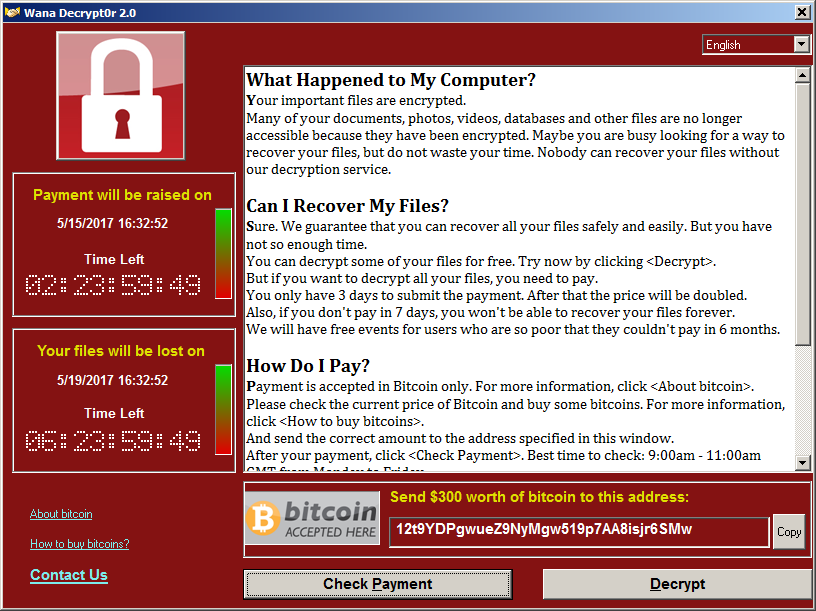
\includegraphics[width=1\textwidth]{wannacry.png}
  \caption{Screenshot of the ransom note left on an infected system}
  \label{fig:wannacry}
\end{figure}
\FloatBarrier
\noindent
\cite{Furnell2017} stated that 200,000 computers across 150 countries were infected, making this the greatest ransomware attack in history (until now). WannaCry used a complex exploit called \textit{EternalBlue}, presumably stolen from \textit{NSA}, to gain access to \textit{Microsoft Windows} operating systems. This may sound very complicated and it is, but malwares can spread very quickly and easily also through trivial phishing attacks. Is important to notice that a ransomware widespread inside an organization may stop its whole business process (temporarily or not) and cost huge amount of money or lives if it blocks critical infrastructures like hospitals.

\subsubsection{Password Attacks}
Suppose we are the manager of a bank: we hire a security team for each entrance, we install cameras and metal detectors, we build an impenetrable vault connected to an alarm system. We think we are safe and sleep soundly. The next day we get up, go to work and find we have been robbed. How was this possible? We discover that we have left the pass code that disable all security measures in plain sight on our computer and the cleaning lady has sold it to some villain that attacked us during the night. This hilarious example does not differ too much from reality: we can install dozens of security procedures, firewalls and things like that, but discovering the control password makes them completely useless. Password attacks can be performed in multiple ways, from brute force on a database to social engineering or simply stealing a sticky note from the desk of a dumb employee. Because of this is important to add an additional layer of security inside any organization: training and security awareness of staff.

\section{...require modern solutions}
Modern organizations deal mostly with data and digital information or at least use IT means to manage and control their businesses. For this reason they require new ways to protect their assets. Risk management evolved to cyber risk management and in the same way standards and best practices have adapted to the new needs. The \textit{International Organization for Standardization} (ISO) jointly with the \textit{International Electrotechnical Commission} (IEC) published the ISO/IEC 27000-series that comprises information security standards, while at national level (US) the \textit{National Institute of Standards and Technology} (NIST) introduced the \textit{NIST Cyber Security Framework} (NIST CSF).\newline
National Security Agency director and head of United States’ Cyber Command Admiral Mike Rodger in 2015 said \textit{“It’s not about if you will be penetrated, but when”} and this is linked to what has been emphasized in \cite{Marvell2015}: understanding the risks and measuring them in real-time is fundamental and put the basis for the whole discipline. How to choose the right solution is up to the Cyber Security Manager, a new figure increasingly present in modern companies whose main purpose is to "prevent rather than cure". What is certain, in fact, is that cyber security is now a fundamental part of organizations, integrated into the various processes and projects since their embryonic stages, the so-called "security by design". The tools available to the sheriff are no longer guns and rifles, but the skills matured in the course of time in this field and the research for advanced methodologies that aim to reduce the occurrences of threats and their impact. There are many new means developed through the years to assist professionals in this sector: they can be software or hardware tools like \textit{Firewalls} and \textit{Intrusion Detection Systems} (IDS) or groups of experts, internal or external to the organizations, like \textit{Security Operation Center} (SOC) or \textit{Computer Security Incident Response Team} (CSIRT). More details in next chapters.
